\scanpage{4}
\margin{transitivité \ldots\\ $R^i f_*$\\ \uline{Suite spectrale de Leray}}
\margin{\ldots}

4°) Foncteurs fibres

Soit $\xi$ un pt géométrique de $X$
\[
\xi\longrightarrow X,\quad\text{d'où foncteur fibre}
\]
\[
u^*:\widetilde X_{\mathrm{ét}}\longrightarrow\widetilde\xi_{\mathrm{ét}}\simeq(\operatorname{Ens})
\]
La famille des foncteurs fibres est \uline{conservative} : $u:F\unsure{-|\longrightarrow}G$ est un isom ssi les $u_{\bar x}:F_{\bar x}\unsure{-|\longrightarrow}G_{\bar x}$ le sont pour $\forall x\in X$.

d'où les cor. habituels.
\[
F_\xi=\underset{\substack{X'\text{ étale sur}\\X\text{ et pointé}\\\text{par }\xi}}{\unsure{\varinjlim}}F(X')
\]

5°) Localisation stricte
\diagram{\begin{tikzcd}
X' \arrow[d] & \xi \arrow[l] \arrow[dl]\\
X &
\end{tikzcd}}
\[
\underline{\mathcal O}_{X,\xi}\ \deleted{\unsure{\mathcal O_X}}
=\underset{\substack{X'\text{ étale sur}\\X\text{ et }\xi\text{-pointé}}}
{\unsure{\mathop{\mathrm{Lim}}\limits_{\longleftrightarrow}}}
\Gamma(X',\mathcal O_{X'})
\]
\margin{$\left.\begin{array}{l}\text{anneaux stricts}\\\text{locaux ou}\\\text{strict local}\end{array}\right\}\Rightarrow$
i.e. \deleted{\unsure{hensélien et}} hensélien et à corps rés. sép. clos}
\[
\bar X^\xi=\operatorname{Spec}\mathcal O_{X,\xi}
\]
\[
F_\xi=\Gamma(\bar X,F_{\bar X})
\]

6°) Application aux fibres des $R^q f_*(F)$ ; pour $f$ qu. cpt. et qu. sép.

\margin{\uline{NB} 5° et 6° \unsure{n'a} pas vraiment d'analogue \unsure{complet} dans le cas des espaces top. ordinaires \ldots}

\figure{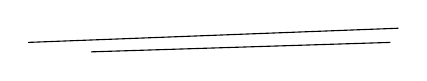
\begin{tikzpicture}
\draw (0,0)--(4.7,0.18);
\draw (0.8,-0.12)--(4.6,0);
\end{tikzpicture}}

7°) \uuline{Théorème fondamental} Soit $f:X\longrightarrow Y$ un morphisme propre, $F$ faisceau \uline{de torsion} sur $X$, alors la formation des $R^i f_*(F)$
\mspage{3}
